\subsection{Visualisierung der Partikelmengen des Partikelfilters}
Da die im Partikelfilter integrierte Visualisierung der Partikelmenge
nicht immer funktionierte und es auch keine direkte Speichermöglichkeit der
 Bilder gab, haben wir den Partikelfilter, so erweitert, dass die
Partikelmenge in eine Datei geschrieben werden kann (
\ref{sec:sonarparticlefilter}) und passend dazu ein Skript (in Python unter
 Benutzung von pygame geschrieben), welches die Partikel anhand der Daten
 aus einer Partikelmengendatei über ein Bild legt. Dieses ist im Ordner
 Visualisierung im SVN-Repository unter dem Namen visualize.py zu finden.
Wir beschreiben im Folgenden zunächst die Installation und Nutzung des
Skriptes, bevor wir auf die Interpretation der Visualisierung eingehen
 \subsubsection{Installieren der Abhängigkeiten des
Visualisierungsskriptes und Benutzung des Skriptes}
 \begin{itemize}
	 \item Python 3.2 herunterladen und installieren\footnote{http://python.org/ftp/python/3.2.2/python-3.2.2.msi}
	 \item pygame 1.9.2a0 für Python 3.2 installieren \footnote{http://pygame.org/ftp/pygame-1.9.2a0.win32-py3.2.msi}
	 \item Python 3.2 zum PATH hinzufügen
	 \item cmd/Eingabeaufforderung öffnen
	 \item In den Ordner Visualisierung des Repositories wechseln
	 \item Das Visualisierungsskript kann nun folgendermaßen benutzt werden:\\
	 		\lstinline|python visualize.py (Dateiname des Bildes) (Dateiname der Partikelmengendatei)| \\
 			z.b. \lstinline|python visualize.py OccuMap.bmp visual.log|
	 \item Das Ausgabebild hat dann den Namen V\_(Dateiname der Partikelmengendatei)\_(Dateiname des Bildes)
\end{itemize}
\subsubsection{Interpretation der Visualisierung}
In den folgenden Bildern sieht man jeweils die Partikelverteilung, wie
sie sich nach der initalen $360^{\circ}$-Rotation zur
Partikelfilter-Initialisierung darstellt. In den oberen beiden Bildern
wurde dabei der Roboter an der linken respektive rechten Wand des
Raums gestartet, in den unteren beiden in der linken respektive
rechten Hälfte der Raummitte:
\begin{nofloat}{figure}
 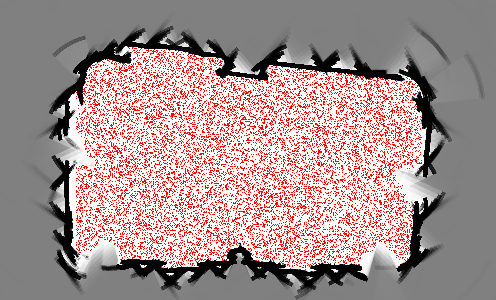
\includegraphics[width=0.5\linewidth]{bilder/visualisierung/visualisierung2}
 \
 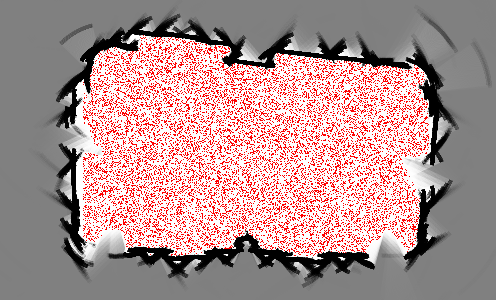
\includegraphics[width=0.5\linewidth]{bilder/visualisierung/visualisierung3}
 \caption{Partikelverteilung im Partikelfilter bei Start nahe der Wände}
\end{nofloat}
\begin{nofloat}{figure}
 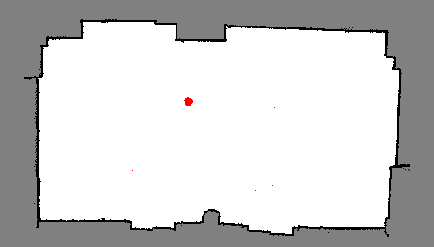
\includegraphics[width=0.5\linewidth]{bilder/visualisierung/visualisierung4}
 \
 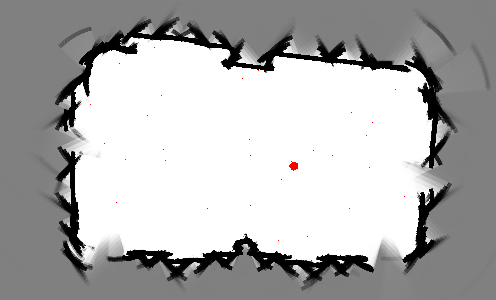
\includegraphics[width=0.5\linewidth]{bilder/visualisierung/visualisierung5}
  \caption{Partikelverteilung im Partikelfilter bei Start in der Raummitte}
\end{nofloat} 

In den oberen beiden Bildern sind die Partikel auf der gesamten
Raumkarte verteilt, somit ist es unmöglich aus einer Partikelhäufung
auf eine bestimmte Position des Roboters im Raum zu schließen. In der
Tat entsprach bei unseren Versuchen die vom Client an den Server
übergebene Position nur in seltenen Fällen der Tatsächlichen, wenn wir
wie in den beiden dargestellten Fällen, den Client an den Wänden des
Raumes gestartet haben. Haben wir hingegen, wie in den unteren beiden
Fällen, eine Position nahe der Raummitte gewählt, erzielten wir im
Allgemeinen sehr gute Ergebnisse für die initiale Position des
Roboters auf der Karte. Sie entsprach meistens der Tatsächlichen. Dies
ist wenig überraschend, wenn man die Visualisierung betrachtet: Es ist
eine klare Konzentration der Partikel auf die Startposition des
Roboters zu beachten. \\\\
Ob im weiteren Verlauf der Ballsuche brauchbare Ergebnisse bei der
Lokalisierung kamen, war analog stark von der initialen Lokalisierung
abhängig: War schon die Startposition falsch, änderte sich dies
auch nicht im Verlauf der Ballsuche. War sie hingegen richtig, wurden
in der Folge auch die weiteren Positionen korrekt bestimmt. Trotzdem
kam es mitunter, insbesondere wenn sich der Roboter in der Nähe von
Raumecken oder Wänden aufhielt zu Sprüngen. Die 
vorhandenen Sprünge sind in einen akzeptablen Rahmen, der die
Funktionsweise des Clients nicht gefährdet.
%Der weitere Verlauf der Ballsuch
%%% Local Variables:
%%% mode: latex
%%% TeX-master: "template"
%%% End:
